% !TeX program = lualatex
% !TeX encoding = utf8
% !TeX spellcheck = uk_UA
% !TeX root = ../EMConspect.tex
% УВАГА: для \enquote{...} потрібен пакет csquotes (\usepackage[ukrainian=quotes]{csquotes}
% в преамбулі EMConspect.tex) --- переконайтесь, що він підключений.

%=========================================================
\chapter{Електричне поле у діелектриках}\label{\currfilebase}
\graphicspath{{\currfilebase/Pictures}}
%=========================================================
\epigraph{Речовина в електричному полі --- це не пасивне тло, а активний співучасник взаємодії: поле поляризує речовину, а речовина, у відповідь,
	послаблює поле.
}{Переосмислення ідей сучасної фізики}


%% --------------------------------------------------------
\section{Основні поняття}
%% --------------------------------------------------------

Досі ми розглядали електричне поле у вакуумі та у провідниках. У провідниках, як ми з'ясували, вільні заряди --- електрони --- під дією як завгодно
слабкого поля переміщуються на макроскопічні відстані, аж доки поле всередині провідника не звернеться в нуль. Проте більшість речовин, що оточують
нас, --- скло, вода, повітря, пластмаси, --- поводяться зовсім інакше: внесені в електричне поле, вони не гасять його всередині себе, а лише
\emphx{послаблюють}. Такі речовини називають \emphx{діелектриками}.

Відмінність діелектрика від провідника пов'язана з тим, які заряди є в його структурі. Домовимось умовно розділяти всі заряди речовини на два типи.

\begin{enumerate}
	\item \emphx{Вільні заряди} --- це заряди, які можуть переміщатися на великі відстані в речовині (набагато більші за міжатомні відстані). Саме
	      вільні заряди відповідають за струм і за повну компенсацію зовнішнього поля всередині провідника. У діелектриках вільних зарядів, як
	      правило, дуже мало, або немає зовсім.
	\item \emphx{Зв'язані (поляризаційні) заряди} --- це заряди, які під дією зовнішніх полів або сил лише незначно \emphx{зміщуються} відносно
	      свого положення рівноваги (електрон у атомі, іон у вузлі кристалічної ґратки) і повертаються назад, у положення рівноваги, одразу після
	      зняття зовнішнього впливу.
\end{enumerate}

\begin{Attention}
	\emphx{Діелектриками} називають речовини, в структурі яких є зв'язані заряди, а вільних зарядів дуже мало або зовсім немає. На відміну від
	провідників, у діелектриках немає носіїв заряду, здатних переміщатися по всьому об'єму тіла: усі заряджені частинки --- електрони та ядра ---
	міцно утримуються в межах свого атома чи молекули.
\end{Attention}

\subsection*{Мікроскопічне та макроскопічне поле}

Щоб коректно описати поведінку речовини в полі, потрібно спершу з'ясувати, про яке саме поле йдеться. Якщо подивитись на речовину на атомному
масштабі, електричне поле виявляється надзвичайно нерівномірним: всередині атома чи молекули воно на багато порядків сильніше, ніж у проміжку між
молекулами, і різко змінюється від точки до точки та в часі --- адже електрони рухаються, атоми коливаються. Таке істинне, швидкозмінне поле
називають \emphx{мікрополем} $\Efield_\text{micro}$.

Усі макроскопічні прилади --- вольтметри, зонди, наші вимірювання --- фізично не здатні відстежити настільки швидкі та дрібномасштабні варіації поля.
Те, що вони фіксують, --- це поле, усереднене по деякому \emphx{фізично нескінченно малому об'єму} $\Delta V$: досить малому порівняно з розмірами
тіла, щоб вважатися \enquote{точкою} в макроскопічному сенсі, але водночас достатньо великому, щоб містити величезну кількість атомів і молекул. Таке
\emphx{середнє (макроскопічне) поле} визначається як
\begin{equation}\label{eq:AvgField}
	\tcbhighmath{
		\left\langle \Efield\right\rangle = \frac1{\Delta V} \iiint\limits_{\Delta V} \Efield_\text{micro}\, dV.
	}
\end{equation}

Це поле змінюється в просторі істотно повільніше, ніж мікрополе, і саме його ми надалі й називатимемо просто $\Efield$, коли говоритимемо про поле
всередині речовини.

%% --------------------------------------------------------
\section{Структура діелектриків}
%% --------------------------------------------------------

\subsection*{Дипольні моменти молекул}

За відсутності зовнішнього поля позитивний заряд ядер атомів, що утворюють молекулу, і негативний заряд електронної оболонки в сумі дають нуль, тобто
молекула електронейтральна. Проте розподіл цих зарядів у просторі не завжди симетричний. Якщо \enquote{центр ваги} позитивного заряду молекули не збігається
з \enquote{центром ваги} негативного, молекула має власний, сталий \emphx{дипольний момент} $\vect p_0$. Причиною такої асиметрії є \emphx{різна
	електронегативність} атомів, що входять до складу молекули: атом з більшою електронегативністю сильніше \enquote{притягує} до себе спільну електронну
хмару, і на ньому виникає надлишок негативного заряду, тоді як на іншому атомі --- надлишок позитивного.

Молекули з ненульовим власним дипольним моментом називають \emphx{полярними}. Класичний приклад --- молекула води $\ce{H2O}$: через кутову форму
молекули (кут між зв'язками O--H становить приблизно $105^\circ$) дипольні моменти окремих зв'язків O--H не компенсують одне одного, і молекула в
цілому має досить великий дипольний момент (рис.~\ref{pic:MoleculeDipoles}).

\begin{figure}[h!]\centering
	\localinput{moleculedipole.tikz}
	\caption{Власні дипольні моменти молекул $\ce{H2O}$ та $\ce{NH3}$\label{pic:MoleculeDipoles}}
\end{figure}

Для вимірювання дипольних моментів молекул зручно користуватись позасистемною одиницею --- \emphx{дебаєм} (позначається \textit{Д} або \textit{D}),
названою на честь фізика П.~Дебая:
\begin{equation*}
	1\ \text{Дебай} = 10^{-18}\ \text{Фр}\cdot\text{см}.
\end{equation*}
Більшість полярних молекул має дипольний момент порядку $1$ Д. Одиниця широко застосовується у фізичній хімії, атомній і молекулярній фізиці.
Дипольні моменти деяких відомих полярних молекул наведено в таблиці~\ref{tab:dipoles}.

\begin{table}[h!]
	\centering
	\caption{Дипольні моменти деяких полярних молекул\label{tab:dipoles}}
	\begin{tabular}{lc}
		\toprule
		Молекула                    & Дипольний момент (Дебай) \\
		\midrule
		Вода ($\ce{H2O}$)           & 1.84                      \\
		Аміак ($\ce{NH3}$)          & 1.46                      \\
		Вуглекислий газ ($\ce{CO2}$) & 0.00                     \\
		Хлороводень ($\ce{HCl}$)    & 1.08                      \\
		Метанол ($\ce{CH3OH}$)      & 1.70                      \\
		\bottomrule
	\end{tabular}
\end{table}

Показовим є приклад вуглекислого газу $\ce{CO2}$: незважаючи на те, що кожен зв'язок C=O є полярним, молекула лінійна і симетрична, тому дипольні
моменти окремих зв'язків повністю компенсують одне одного, і сумарний дипольний момент молекули дорівнює нулю.

\subsection*{Неполярні молекули та наведений дипольний момент}


\emphx{Неполярні молекули} --- це молекули, в яких електричні заряди розподілені симетрично, і власний дипольний момент відсутній ($p_0 = 0$).
У таких молекулах атоми зазвичай мають однакову або близьку електронегативність, тому спільна електронна хмара розподілена рівномірно між
атомами, або ж молекула має достатньо високу симетрію (як у випадку $\ce{CO2}$). Прикладами неполярних молекул є кисень $\ce{O2}$, азот
$\ce{N2}$, метан $\ce{CH4}$, а також окремі атоми інертних газів.


Важливо розуміти, що відсутність \emphx{власного} дипольного моменту не означає, що неполярна молекула взагалі не може мати дипольного моменту. У
зовнішньому електричному полі позитивно заряджене ядро і негативно заряджена електронна хмара зміщуються в протилежні боки: ядро --- за полем,
електрони --- проти поля (рис.~\ref{pic:InducedDipole}). В результаті \enquote{центри ваги} позитивного та негативного зарядів розходяться, і в молекулі
виникає \emphx{наведений (індукований) дипольний момент}, пропорційний прикладеному полю:
\begin{equation}\label{eq:InducedDipole}
	\vect p = \alpha \Efield,
\end{equation}
де коефіцієнт $\alpha$ називають \emphx{поляризовністю молекули}.

\begin{figure}[h!]\centering
	\localinput{nonpolar-molecule.tikz}
	\caption{Неполярна молекула без зовнішнього поля та в зовнішньому полі\label{pic:InducedDipole}}
\end{figure} Цей механізм появи дипольного моменту називають \emphx{електронною
	(деформаційною) поляризацією}: оскільки маса електронної хмари набагато менша за масу ядра, саме зміщення електронної хмари відносно ядра і дає
основний внесок у наведений момент. На відміну від орієнтаційного механізму, який ми розглянемо в п.~\ref{sec:Langevin-Debye}, електронна
поляризовність практично не залежить від температури.

%% --------------------------------------------------------
\section{Поляризація діелектриків}
%% --------------------------------------------------------

\begin{Attention}
	\emphx{Поляризація} --- це просторовий \emphx{перерозподіл зв'язаних зарядів}, що призводить до виникнення об'ємного дипольного моменту
	середовища. Поляризація може виникати як під дією зовнішнього електричного поля, так і під впливом інших зовнішніх чинників --- механічної
	деформації, зміни температури тощо.
\end{Attention}

Розглянемо, як відбувається поляризація в двох основних класах діелектриків.

\begin{itemize}
	\item \emphx{Полярні діелектрики} складаються з полярних молекул, кожна з яких уже має власний дипольний момент $\vect p_0 \neq 0$. За
	      відсутності зовнішнього поля теплове (хаотичне) обертання молекул орієнтує їхні дипольні моменти цілком випадково в усіх напрямках, тому в
	      будь-якому фізично малому об'ємі дипольні моменти в середньому взаємно компенсуються, і сумарний дипольний момент речовини дорівнює нулю.
	      Коли ж прикладене зовнішнє поле, воно створює момент сил, що прагне розвернути кожен диполь уздовж поля (див.~формулу
	      $\vect M = [\vect p\times\Efield]$, отриману в попередньому розділі). Тепловий рух заважає ідеальному впорядкуванню, проте певна переважна
	      орієнтація вздовж поля все ж встановлюється --- виникає так звана \emphx{орієнтаційна поляризація}.
	\item \emphx{Неполярні діелектрики} складаються з неполярних молекул, у яких за відсутності поля центри позитивного й негативного зарядів
	      збігаються. Зовнішнє поле зміщує електронні хмари відносно ядер (формула~\eqref{eq:InducedDipole}), і в кожній молекулі виникає наведений
	      дипольний момент, зорієнтований уздовж поля, --- \emphx{електронна поляризація}.
\end{itemize}

% ==================== FIGURE 1: полярні молекули ====================
\begin{figure}[h!]
	\centering
	% --- (а) кадр 1: полярні молекули без поля ---
	\begin{subfigure}[t]{0.48\linewidth}
		\centering
		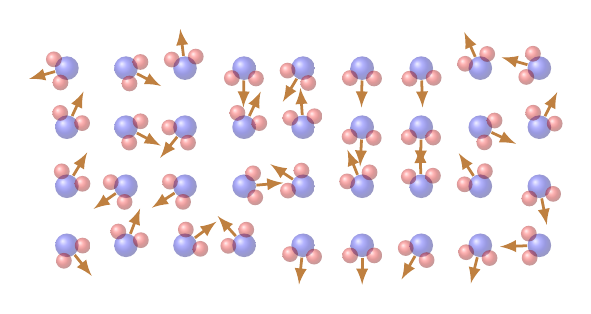
\begin{tikzpicture}[>=latex]
			\pgfmathsetseed{1}
			\tikzset{
				water/.pic={
						\begin{scope}[opacity=0.4]
							\node[circle, ball color=blue, inner sep=0, minimum size=0.3cm] (O) at
							(0,0) {};
							\node[circle, ball color=red, inner sep=0, minimum size=0.2cm] (H1) at
							(-50:0.2) {};
							\node[circle, ball color=red, inner sep=0, minimum size=0.2cm] (H2) at
							(50:0.2) {};
						\end{scope}
						\draw[-latex, brown, line width=1pt] (O) -- ++(0.5, 0);
					},
			}
			\foreach \x in {0,...,8}
				{
					\foreach \y in {0,...,3}{
							\pic[rotate={random(0,360)}] at ({0.75*\x}, {0.75*\y}) {water};
						}
				}
		\end{tikzpicture}
		\caption{Без поля}
		\label{pic:PolarNoField}
	\end{subfigure}\hfill
	% --- (б) кадр 2: полярні молекули в полі ---
	\begin{subfigure}[t]{0.48\linewidth}
		\centering
		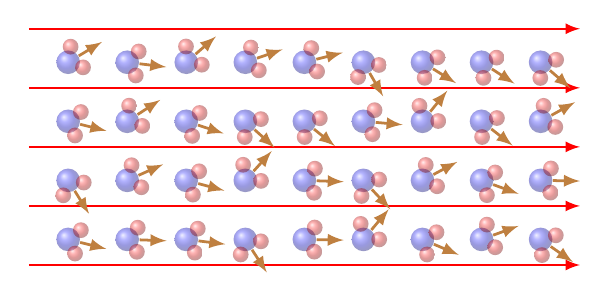
\begin{tikzpicture}[>=latex]
			\pgfmathsetseed{1}
			\tikzset{
				water/.pic={
						\begin{scope}[opacity=0.4]
							\node[circle, ball color=blue, inner sep=0, minimum size=0.3cm] (O) at
							(0,0) {};
							\node[circle, ball color=red, inner sep=0, minimum size=0.2cm] (H1) at
							(-50:0.2) {};
							\node[circle, ball color=red, inner sep=0, minimum size=0.2cm] (H2) at
							(50:0.2) {};
						\end{scope}
						\draw[-latex, brown, line width=1pt] (O) -- ++(0.5, 0);
					},
			}
			\foreach \y in {0,...,4} {
					\draw[->, red, thick] (-0.5,{0.75*\y-0.325}) -- ++(7,0);
				}
			\foreach \x in {0,...,8}
				{
					\foreach \y in {0,...,3}{
							\pic[rotate={random(-60,60)}] at ({0.75*\x}, {0.75*\y}) {water};
						}
				}
		\end{tikzpicture}
		\caption{У полі}
		\label{pic:PolarField}
	\end{subfigure}
	\caption{Поляризація полярних молекул: у зовнішньому електричному полі
		диполі орієнтуються вздовж поля}
	\label{pic:PolarizationPolar}
\end{figure}

% ==================== FIGURE 2: неполярні молекули ====================
\begin{figure}[h!]
	\centering
	% --- (а) кадр 3: неполярні молекули без поля ---
	\begin{subfigure}[t]{0.48\linewidth}
		\centering
		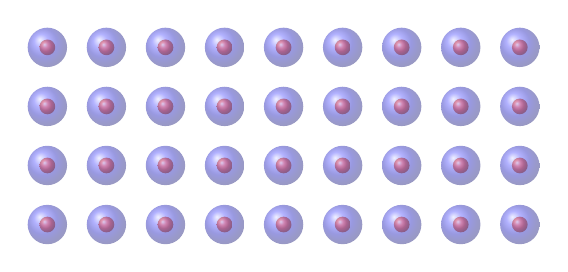
\begin{tikzpicture}[>=latex]
			\tikzset{
				unperturbed/.pic={
						\begin{scope}[opacity=0.4]
							\node[circle, ball color=blue, inner sep=0, minimum size=0.5cm] (O) at
							(0,0) {};
							\node[circle, ball color=red, inner sep=0, minimum size=0.2cm] (H1) at
							(0,0) {};
						\end{scope}
					},
			}
			\foreach \x in {0,...,8}
				{
					\foreach \y in {0,...,3}{
							\pic[] at ({0.75*\x}, {0.75*\y}) {unperturbed};
						}
				}
		\end{tikzpicture}
		\caption{Без поля}
		\label{pic:NonPolarNoField}
	\end{subfigure}\hfill
	% --- (б) кадр 4: неполярні молекули в полі ---
	\begin{subfigure}[t]{0.48\linewidth}
		\centering
		\begin{tikzpicture}[>=latex]
			\tikzset{
				perturbed/.pic={
						\begin{scope}[opacity=0.4]
							\node[ellipse, ball color=blue, inner sep=0, minimum width=0.6cm,
								minimum height=0.4cm] (O) at
							(-0.1,0) {};
							\node[circle, ball color=red, inner sep=0, minimum size=0.2cm] (H1) at
							(+0.02,0) {};
						\end{scope}
						\draw[-latex, brown, line width=1pt] (-0.2,0) -- ++(0.5, 0);
					},
			}
			\foreach \y in {0,...,4} {
					\draw[->, red, thick] (-0.5,{0.75*\y-0.325}) -- ++(7,0);
				}
			\foreach \x in {0,...,8}
				{
					\foreach \y in {0,...,3}{
							\pic[] at ({0.75*\x}, {0.75*\y}) {perturbed};
						}
				}
		\end{tikzpicture}
		\caption{У полі}
		\label{pic:NonPolarField}
	\end{subfigure}
	\caption{Поляризація неполярних молекул: у зовнішньому електричному полі
		молекули деформуються, утворюючи індукований дипольний момент}
	\label{pic:PolarizationNonPolar}
\end{figure}

У випадку йонних кристалів (наприклад, $\ce{NaCl}$) існує ще один механізм --- \emphx{йонна поляризація}: позитивні та негативні йони кристалічної
ґратки під дією поля зміщуються один відносно одного як цілі підґратки, що також створює об'ємний дипольний момент.

В обох випадках --- полярних і неполярних діелектриків --- результат один: на межах виділеного в речовині об'єму з'являються надлишкові
(некомпенсовані) зв'язані заряди, тоді як в основному об'ємі речовини позитивні та негативні заряди сусідніх диполів взаємно компенсують одне одного.
Саме ці надлишкові поверхневі заряди і створюють власне поле речовини $\Efield'$, яке, за принципом суперпозиції, додається до зовнішнього поля
$\Efield_\text{ex}$:
\begin{equation*}
	\Efield = \Efield_\text{ex} + \Efield'.
\end{equation*}
Оскільки диполі орієнтуються так, що їхні позитивні полюси \enquote{дивляться} за полем, а негативні --- проти поля, власне поле $\Efield'$ спрямоване
\emphx{назустріч} зовнішньому, і сумарне поле в діелектрику завжди \emphx{послаблюється} порівняно з зовнішнім.

На рисунку~\ref{pic:PolarizedDielectric} схематично показано поляризований
діелектрик у зовнішньому електричному полі: на протилежних поверхнях
виділеного об'єму виникають некомпенсовані зв'язані заряди $-Q$ та $+Q$,
власне поле яких спрямоване назустріч зовнішньому.



\begin{figure}[h!]
	\centering
	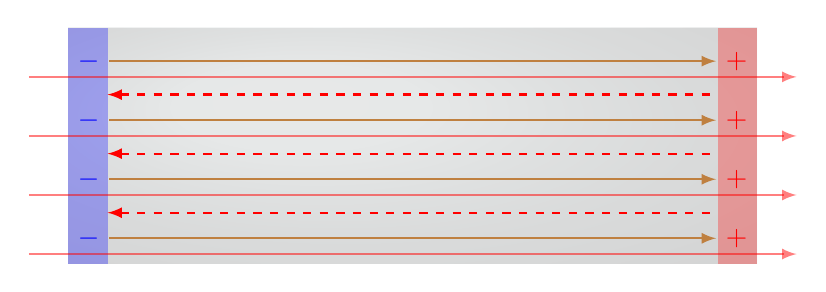
\begin{tikzpicture}[>=latex]
		\begin{scope}
			\fill[ball color=cyan!10, opacity=0.1] (-0.5,{0.75*0-0.325}) rectangle
			++(8.75,{0.75*4});
			\fill[blue, opacity=0.3] (-0.5,{0.75*0-0.325}) rectangle ++(0.5, {0.75*4});
			\fill[red, opacity=0.3] (7.75,{0.75*0-0.325}) rectangle ++(0.5, {0.75*4});
		\end{scope}
		\foreach \y in {0,...,3} {
				\path[] (-0.5,{0.75*\y}) node[right, text=blue] (-Q) {$-$} ++(8.75,0)
				node[left, text=red] (+Q) {$+$};
				\draw[->, brown, thick] (-Q) -- (+Q);

				\ifnum\y<3
					\draw[<-, red, thick, dashed] (0,{0.75*\y+0.325}) -- ++(7.75,0);
				\fi

				\draw[->, red, thick, opacity=0.5] (-1,{0.75*\y-0.2}) -- ++(9.75,0);
			}
	\end{tikzpicture}
    \caption{Поляризований діелектрик у зовнішньому електричному полі:
    	на поверхнях виникають зв'язані заряди $-Q$ та $+Q$. Срілки означають:
    	\protect\tikz[baseline=-0.6ex]{\protect\draw[->, red, thick, opacity=0.5] (0,0) -- (0.6,0);}
    	--- зовнішнє поле $\Efield_\text{ex}$;
    	\protect\tikz[baseline=-0.6ex]{\protect\draw[<-, red, thick, dashed] (0,0) -- (0.6,0);}
    	--- поле зв'язаних зарядів $\Efield'$;
    	\protect\tikz[baseline=-0.6ex]{\protect\draw[->, brown, thick] (0,0) -- (0.6,0);}
    	--- вектор поляризації $\vect{P}$ (також співпадає з результуючим полем $\Efield$).
    }
	\label{pic:PolarizedDielectric}
\end{figure}

\subsection*{Електрострикція}

Уміщення діелектрика в електричне поле призводить не лише до поляризації, а й до \emphx{зміни розмірів тіла}. Це явище називають
\emphx{електрострикцією}, і воно, хоч і різною мірою, спостерігається в усіх без винятку діелектриках. Головні особливості електрострикції:

\begin{enumerate}
	\item деформація не залежить від \emphx{напрямку} поля --- якщо поле змінити на протилежне, деформація не змінить знака. Це прямо пов'язано з
	      тим, що ефект пропорційний \emphx{квадрату} поля $E^2$;
	\item деформація пропорційна квадрату напруженості поля, $\Delta \ell \sim E^2$, тому при збільшенні поля деформація зростає значно швидше, ніж
	      лінійно;
	\item у переважній більшості матеріалів електрострикційний ефект виражений слабко порівняно з п'єзоефектом (див.~п.~\ref{sec:PiezoPyro}), і для
	      отримання помітної деформації потрібне дуже сильне електричне поле.
\end{enumerate}
Отже, електрострикція --- це нелінійна, квадратична за полем і, як правило, малопомітна деформація діелектрика, яка не залежить від напрямку
прикладеного поля.

%% --------------------------------------------------------
\section{Вектор поляризації}
%% --------------------------------------------------------

Для кількісного опису стану поляризованого діелектрика вводять \emphx{макроскопічну} характеристику --- \emphx{вектор поляризації} (або
\emphx{поляризованість}), який дорівнює дипольному моменту одиниці об'єму речовини:
\begin{equation}\label{eq:Pdef}
	\tcbhighmath{
		\vect P = \frac1V \sum_i \vect p_i,
	}
\end{equation}
де підсумовування проводиться за всіма молекулярними диполями $\vect p_i$, що потрапляють у фізично малий об'єм $V$.

Для великого класу діелектриків, що не надто відрізняються за своїми властивостями від вакууму (гази, більшість рідин та аморфних твердих тіл за не
надто сильних полів), експериментально встановлено, що поляризованість лінійно залежить від напруженості поля \emphx{в самому діелектрику}:
\begin{equation}\label{eq:PlinearE}
	\tcbhighmath{
		\vect P = \chi \Efield,
	}
\end{equation}
де безрозмірна величина $\chi > 0$ називається \emphx{поляризовністю речовини} (у частині літератури цю ж величину називають \emphx{діелектричною
сприйнятливістю} --- термін цілком рівноправний, проте надалі ми користуватимемось терміном \enquote{поляризовність}, підкреслюючи його спорідненість
з поляризовністю окремої молекули $\alpha$, формула~\eqref{eq:InducedDipole}: перша --- мікроскопічна, друга --- макроскопічна характеристики того
самого явища, а нетривіальний зв'язок між ними --- предмет п.~\ref{sec:AtomPolarizability} і п.~\ref{sec:ClausiusMossotti}). Поляризовність $\chi$
не залежить від $\Efield$ і характеризує властивості самого діелектрика (тип молекул, їхню концентрацію, температуру тощо). Такі діелектрики
називають \emphx{лінійними}.

\begin{Attention}
	Не всі діелектрики є лінійними. Існують діелектрики, для яких співвідношення $\vect P = \chi\Efield$ не виконується: деякі йонні кристали,
	електрети, а особливо --- сегнетоелектрики, для яких зв'язок між $\vect P$ і $\Efield$ нелінійний і до того ж неоднозначний (див.~п.~\ref{sec:FE}).
\end{Attention}

\subsection*{Тензор поляризовності. Нелінійні діелектрики}

Формула~\eqref{eq:PlinearE} має два принципові обмеження. По-перше, вона передбачає, що вектор поляризації $\vect P$ завжди паралельний полю
$\Efield$, з однаковим коефіцієнтом пропорційності за будь-якого напрямку поля. Це справедливо лише для \emphx{ізотропних} середовищ --- газів,
рідин, аморфних тіл, полікристалів без переважної орієнтації зерен. У кристалах же, структура яких не має сферичної симетрії, відгук речовини на
поле, взагалі кажучи, залежить від напрямку: поле, прикладене вздовж однієї кристалографічної осі, породжує не лише поляризацію вздовж цієї осі, а
й певні складові вздовж інших осей. У такому разі кожна компонента вектора $\vect P$ лінійно виражається через \emphx{усі} компоненти поля:
\begin{equation}\label{eq:PolTensorLinear}
	\tcbhighmath{
		P_i = \sum_j \chi_{ij}\, E_j, \qquad i,j = x,y,z,
	}
\end{equation}
де сукупність дев'яти величин $\chi_{ij}$ утворює симетричний тензор другого рангу, який називають \emphx{тензором поляризовності} речовини (за
аналогією з поляризовністю окремої молекули, формула~\eqref{eq:InducedDipole}). Симетричність $\chi_{ij}=\chi_{ji}$ --- не випадковість, а наслідок
термодинамічної оборотності процесу поляризації (так само, як симетричним є тензор інерції). Для ізотропного діелектрика цей тензор вироджується в
скалярну величину, $\chi_{ij} = \chi\,\delta_{ij}$, і формула~\eqref{eq:PolTensorLinear} зводиться до вже знайомої~\eqref{eq:PlinearE}.

\begin{Attention}
	Ізотропними за поляризовністю є не лише аморфні тіла та рідини, а й кристали \emphx{кубічної} сингонії: попри те, що їхня ґратка анізотропна (і,
	наприклад, пружні властивості кубічного кристала залежать від напрямку), висока симетрія кубічної ґратки виявляється достатньою, щоб тензор
	$\chi_{ij}$ звівся до скаляра. Усі кристали \emphx{нижчої} симетрії (тетрагональні, гексагональні, ромбічні, моноклінні, триклінні) --- уже
	справді анізотропні за $\chi_{ij}$, і формулу~\eqref{eq:PolTensorLinear} для них слід використовувати в повному, тензорному вигляді.
\end{Attention}

По-друге, формула~\eqref{eq:PlinearE} --- це лише перший, лінійний член у більш загальній залежності $\vect P(\Efield)$. У достатньо сильних полях
(наприклад, у полі потужного лазерного випромінювання) внесок вищих степенів поля вже не можна знехтувати, і поляризацію слід записувати у вигляді
ряду за степенями $\Efield$:
\begin{equation}\label{eq:NonlinearP}
	\tcbhighmath{
		P_i = \sum_j \chi^{(1)}_{ij} E_j + \sum_{jk} \chi^{(2)}_{ijk} E_j E_k + \sum_{jkl} \chi^{(3)}_{ijkl} E_j E_k E_l + \ldots,
	}
\end{equation}
де $\chi^{(1)}_{ij}$ --- уже знайомий (лінійний) тензор поляризовності~\eqref{eq:PolTensorLinear}, а $\chi^{(2)}_{ijk}$, $\chi^{(3)}_{ijkl}$, \dots
--- тензори поляризовності вищих порядків (другого, третього тощо). Їхні компоненти, як правило, на багато порядків менші за компоненти
$\chi^{(1)}_{ij}$, тому внесок нелінійних доданків стає помітним лише за дуже сильних полів. Діелектрики, для яких доводиться враховувати ці
доданки, називають \emphx{нелінійними}. \textit{Застереження:} тут ряд~\eqref{eq:NonlinearP} записано в найпростішому, \enquote{миттєвому}
(квазістатичному) наближенні --- лише щоб показати структуру нелінійного відгуку; у строгій нелінійній оптиці кожен $\chi^{(n)}$ додатково залежить
від частот взаємодіючих хвиль і має свої комбінаторні множники, що виходить за межі цього курсу.

\begin{Attention}
	Тензор поляризовності другого порядку $\chi^{(2)}_{ijk}$ тотожно дорівнює нулю в будь-якому середовищі, що має центр симетрії (так само, як і
	п'єзоефект, див.~п.~\ref{sec:PiezoPyro}): інверсія поля $\Efield \to -\Efield$ у центросиметричному кристалі повинна давати $\vect P \to -\vect
	P$, а квадратичний за полем доданок при заміні знака поля свого знака не змінює. Отже, квадратична нелінійність можлива лише в
	нецентросиметричних кристалах --- тих самих, що виявляють п'єзоелектричні властивості.
\end{Attention}

Нелінійна поляризовність лежить в основі \emphx{нелінійної оптики}: доданок з $\chi^{(2)}$ відповідає, зокрема, за \emphx{генерацію другої
	гармоніки} (перетворення лазерного випромінювання частоти $\omega$ у випромінювання подвоєної частоти $2\omega$) та за \emphx{ефект Поккельса}
(лінійну за полем зміну показника заломлення, на якій ґрунтуються електрооптичні модулятори світла). Типові нелінійно-оптичні кристали --- ніобат
літію $\ce{LiNbO3}$, дигідрофосфат калію (KDP), бета-борат барію (BBO). Доданок з $\chi^{(3)}$ відповідає за \emphx{ефект Керра} (квадратичну за
полем зміну показника заломлення) та генерацію третьої гармоніки.

\subsection*{Однорідна та неоднорідна поляризація}

Поляризацію називають \emphx{однорідною}, якщо вектор $\vect P$ є сталим у всьому об'ємі речовини, $\vect P = \const$, і \emphx{неоднорідною}, якщо
$\vect P$ змінюється від точки до точки.

\emphx{Однорідна поляризація.} Нехай поляризація однорідна. Розглянемо косокутний паралелепіпед, вирізаний із поляризованої речовини так, що його
бічне ребро паралельне вектору поляризації $\vect P$ (рис.~\ref{pic:PolarizedParallelepiped}). Якщо $S$ --- площа бічної грані, а $\ell$ --- довжина
ребра паралелепіпеда, то його об'єм дорівнює $V = S\ell\cos\theta$, де $\theta$ --- кут між ребром $\vect \ell$ і нормаллю до бічної грані.

\begin{figure}[h!]\centering
	\localinput{parallelepiped.tikz}
	\caption{Косокутний паралелепіпед, вирізаний з однорідно поляризованого діелектрика уздовж
		вектора поляризації $\vect P$\label{pic:PolarizedParallelepiped}}
\end{figure}

Диполі всередині такого паралелепіпеда шикуються \enquote{голова до хвоста}: позитивний заряд одного диполя сусідить з негативним зарядом наступного, і в
об'ємі речовини ці заряди взаємно компенсуються. Некомпенсованими лишаються тільки заряди на двох торцевих гранях: на одній виступає надлишковий
позитивний заряд, на іншій --- негативний. Тому весь паралелепіпед еквівалентний одному великому диполю з дипольним моментом $\vect p = \sigma' S
	\vect \ell$, де $\sigma'$ --- поверхнева густина \emphx{зв'язаного (поляризаційного)} заряду на торцевій грані. З іншого боку, за
означенням~\eqref{eq:Pdef}, дипольний момент паралелепіпеда дорівнює $\vect p = \vect P \cdot V = \vect P \, S\ell\cos\theta$. Прирівнюючи обидва
вирази і враховуючи, що $\vect P \cdot \vect n = P\cos\theta$ (де $\vect n$ --- зовнішня нормаль до грані), отримуємо просту й важливу формулу:
\begin{equation}\label{eq:SigmaPrime}
	\tcbhighmath{
		\vect P \cdot \vect n = P_n = \sigma'.
	}
\end{equation}

\begin{Attention}
	Нормальна складова вектора поляризації на поверхні діелектрика чисельно дорівнює поверхневій густині зв'язаного заряду, що виступає на цій
	поверхні. Там, де вектор $\vect P$ спрямований \emphx{із} речовини (нормальна складова додатна), на поверхні виступає позитивний зв'язаний
	заряд; там, де $\vect P$ спрямований \emphx{у} речовину, --- негативний.
\end{Attention}

\emphx{Неоднорідна поляризація.} Нехай тепер поляризація неоднорідна, і в товщі речовини виділено об'єм $V$ довільної форми, обмежений замкненою
поверхнею $S$ (рис.~\ref{pic:NonUniformPolarization}). Кожен малий елемент поверхні $dS$ можна, як і вище, вважати гранню елементарного косокутного
паралелепіпеда, тому на ньому виступає поверхневий зв'язаний заряд $d q' = \sigma' dS = P_n\, dS$.

\begin{figure}[h!]\centering
	\localinput{nonuniform-polarization.tikz}
	\caption{Довільний об'єм неоднорідно поляризованого діелектрика: на поверхні виступають
		некомпенсовані зв'язані заряди\label{pic:NonUniformPolarization}}
\end{figure} Підсумовуючи (інтегруючи) цей вираз за всією замкненою поверхнею, знаходимо повний
заряд, що вийшов на зовнішню поверхню виділеного об'єму:
\begin{equation*}
	q'_{\text{пов}} = \oiint\limits_S P_n\, dS.
\end{equation*}
Але сама речовина, з якої вирізано цей об'єм, електронейтральна: поляризація лише \emphx{перерозподіляє} наявні заряди, не створюючи нових. Тому
якщо на зовнішню поверхню вийшов заряд $q'_{\text{пов}}$, то всередині об'єму мусив залишитися зв'язаний заряд протилежного знака, розподілений з
об'ємною густиною $\rho'$:
\begin{equation}\label{eq:GaussForP-int}
	\tcbhighmath{
		\oiint\limits_S \vect P\cdot d\vect S = \oiint\limits_S P_n\, dS = - \iiint\limits_V \rho'\, dV.
	}
\end{equation}
Це співвідношення називають \emphx{теоремою Гаусса для вектора поляризації}: воно за формою повністю аналогічне теоремі Гаусса для поля $\Efield$
(п.~\ref{sec:Gauss}), проте зв'язує потік вектора $\vect P$ не з повним, а лише зі \emphx{зв'язаним} зарядом, узятим із протилежним знаком.

Так само, як ми переходили від інтегральної форми теореми Гаусса для $\Efield$ до диференціальної, стягуючи об'єм $V$ у точку, з
формули~\eqref{eq:GaussForP-int} отримуємо \emphx{диференціальну форму теореми Гаусса для вектора поляризації}:
\begin{equation}\label{eq:GaussForP-diff}
	\tcbhighmath{
		\divg \vect P = -\rho'.
	}
\end{equation}
Дивергенція вектора поляризації в даній точці дорівнює об'ємній густині зв'язаного заряду в цій точці, узятій зі знаком мінус. У окремому випадку
однорідної поляризації, коли $\vect P = \const$, маємо $\divg \vect P \equiv 0$, а отже, і $\rho' = 0$: об'ємний зв'язаний заряд в однорідно
поляризованому діелектрику відсутній, увесь надлишковий заряд зосереджений на поверхні, що узгоджується з розглянутим вище прикладом
паралелепіпеда.

%% --------------------------------------------------------
\section{Вектор електричної індукції}\label{sec:Dfield}
%% --------------------------------------------------------

Електричне поле всередині речовини створюється не лише вільними, а й зв'язаними (поляризаційними) зарядами. Тому в теоремі Гаусса для поля
$\Efield$ (яка, нагадаємо, є універсальним законом і виконується для будь-яких зарядів) слід урахувати обидва типи зарядів --- і вільні $\rho$, і
зв'язані $\rho'$:
\begin{equation*}
	\divg \Efield = 4\pi(\rho + \rho').
\end{equation*}
Скориставшись знайденим щойно співвідношенням~\eqref{eq:GaussForP-diff}, а саме $\rho' = -\divg\vect P$, отримуємо:
\begin{equation*}
	\divg \Efield = 4\pi\rho - 4\pi \divg\vect P
	\quad\Longrightarrow\quad
	\divg\left(\Efield + 4\pi \vect P\right) = 4\pi\rho.
\end{equation*}
Вираз у дужках зручно позначити окремим символом і назвати \emphx{вектором електричної індукції}:
\begin{equation}\label{eq:Ddef}
	\tcbhighmath{
		\Dfield = \Efield + 4\pi\vect P.
	}
\end{equation}
Тоді теорема Гаусса для електричного поля \emphx{в речовині} набуває вигляду
\begin{equation}\label{eq:GaussForD-diff}
	\tcbhighmath{
		\divg\Dfield = 4\pi\rho,
	}
\end{equation}
а в інтегральній формі --- відповідно
\begin{equation}\label{eq:GaussForD-int}
	\tcbhighmath{
		\oiint\limits_S \Dfield\cdot d\vect S = 4\pi \iiint\limits_V \rho\, dV.
	}
\end{equation}

\begin{Attention}
	У формулювання теореми Гаусса для поля в речовині входять \emphx{тільки вільні заряди} $\rho$. Внесок зв'язаних (поляризаційних) зарядів уже
	враховано --- він \enquote{захований} усередині означення вектора індукції $\Dfield$. Саме тому вектор $\Dfield$ є надзвичайно зручним інструментом:
	для обчислення його потоку крізь довільну поверхню достатньо знати лише розподіл \emphx{вільних} зарядів, які, на відміну від зв'язаних, як
	правило, відомі заздалегідь (наприклад, задані зарядом на обкладинках конденсатора).
\end{Attention}

Підкреслимо: на відміну від $\Efield$, вектор $\Dfield$ \emphx{не} є потенціальним силовим полем у звичайному розумінні --- він не діє безпосередньо
на пробний заряд. Це допоміжна, суто розрахункова величина, яка водночас має ясний фізичний зміст: вона \enquote{відстежує} тільки ті заряди, якими ми
керуємо ззовні (вільні), незалежно від того, який діелектрик їх оточує.

\subsection*{Діелектрична проникність}

Для лінійних діелектриків, у яких справедливе співвідношення~\eqref{eq:PlinearE}, вектор індукції теж виявляється пропорційним $\Efield$:
\begin{equation*}
	\Dfield = \Efield + 4\pi\vect P = \Efield + 4\pi\chi\Efield = (1+4\pi\chi)\Efield.
\end{equation*}
Позначаючи
\begin{equation}\label{eq:eps}
	\tcbhighmath{
		\epsilon = 1 + 4\pi\chi,
	}
\end{equation}
отримуємо просте й дуже часто використовуване співвідношення
\begin{equation}\label{eq:DepsE}
	\tcbhighmath{
		\Dfield = \epsilon\Efield.
	}
\end{equation}
Величину $\epsilon$ називають \emphx{діелектричною проникністю середовища}. Оскільки для звичайних (не сегнетоелектричних) речовин у постійних полях
завжди $\chi > 0$, то й $\epsilon > 1$: діелектрична проникність будь-якого \enquote{нормального} діелектрика перевищує одиницю. Для вакууму, в якому
поляризація відсутня ($\chi = 0$), маємо $\epsilon = 1$, і вектори $\Dfield$ та $\Efield$ збігаються.

\emphx{Приклад.} Розглянемо точковий заряд $Q$, вміщений у нескінченний однорідний діелектрик з проникністю $\epsilon$ (рис.~\ref{pic:PointChargeDielectric}). Через сферичну симетрію
задачі, за теоремою Гаусса для вектора $\Dfield$, як і у випадку поля у вакуумі,
\begin{equation*}
	\Dfield = \frac{Q}{r^2}\frac{\vect r}{r},
\end{equation*}
а звідси, користуючись~\eqref{eq:DepsE}, знаходимо напруженість поля безпосередньо в діелектрику:
\begin{equation*}
	\Efield = \frac{\Dfield}{\epsilon} = \frac{Q}{\epsilon r^2}\frac{\vect r}{r}.
\end{equation*}
Оскільки $\epsilon > 1$, поле точкового заряду в діелектрику всюди \emphx{слабкіше}, ніж таке саме поле у вакуумі. Це прямий кількісний прояв уже
відомого нам якісного результату: \emphx{поляризаційні заряди, що виникають навколо заряду $Q$, послаблюють його поле}.

\begin{figure}[h!]\centering
	\localinput{point-charge-dielectric.tikz}
	\caption{Точковий заряд у нескінченному однорідному діелектрику\label{pic:PointChargeDielectric}}
\end{figure}

%% --------------------------------------------------------
\section{Граничні умови в присутності діелектриків}
%% --------------------------------------------------------

Як і у випадку поля у вакуумі (п.~\ref{sec:BC}), на межі розділу двох середовищ (двох діелектриків, або діелектрика й вакууму) поле може змінюватись
стрибком. Знайдемо, як пов'язані значення полів по обидва боки межі.

\emphx{Перша гранична умова (для нормальної складової $\Dfield$).} Застосуємо теорему Гаусса для вектора $\Dfield$ до нескінченно малого циліндра,
що охоплює невелику ділянку межі розділу середовищ 1 та 2, так само, як ми робили це для поля $\Efield$ на поверхні провідника (рис.~\ref{pic:BC1}).
Нехай $\sigma$ ---
поверхнева густина \emphx{вільного} заряду на межі розділу (якщо він там є). Враховуючи, що $d\vect S_1 = -d\vect S_2 = \vect n\, dS$, де $\vect n$
--- нормаль, спрямована з середовища 1 у середовище 2, маємо

\begin{figure}[h!]\centering
	\localinput{bc1.tikz}
	\caption{Циліндр Гаусса на межі розділу двох середовищ для виведення граничної умови на
		нормальну складову $\Dfield$\label{pic:BC1}}
\end{figure}
\begin{equation*}
	\oiint\limits_S \Dfield\cdot d\vect S = 4\pi\sigma \, dS
	\quad\Longrightarrow\quad
	\Dfield_2 \cdot d\vect S_2 + \Dfield_1\cdot d\vect S_1 \equiv (D_{2n} - D_{1n})\, dS = 4\pi\sigma\, dS,
\end{equation*}
звідки
\begin{equation}\label{eq:BC1-D}
	\tcbhighmath{
		D_{2n} - D_{1n} = 4\pi\sigma.
	}
\end{equation}

\begin{Attention}
	Нормальна складова вектора $\Dfield$ зазнає стрибка при переході через границю розділу середовищ \emphx{лише за наявності на ній вільних
		зарядів}. Якщо вільних зарядів на межі розділу немає ($\sigma = 0$), то $D_{1n} = D_{2n}$, і стрибка немає --- на відміну від нормальної
	складової $\Efield$, яка, узагалі кажучи, все одно змінюється стрибком через наявність зв'язаних поверхневих зарядів!
\end{Attention}

\emphx{Друга гранична умова (для тангенціальної складової $\Efield$).} Ця умова не пов'язана з наявністю діелектрика і виводиться так само, як і
раніше (п.~\ref{sec:BC}), із теореми про циркуляцію вектора $\Efield$ уздовж нескінченно малого прямокутного контуру $L$, що проходить по обидва боки
межі розділу (рис.~\ref{pic:BC2}); ця теорема залишається справедливою в будь-якому середовищі --- адже електростатичне
поле завжди потенціальне, незалежно від того, вакуум це чи діелектрик:

\begin{figure}[h!]\centering
	\localinput{bc2.tikz}
	\caption{Контур циркуляції на межі розділу двох середовищ для виведення граничної умови на
		тангенціальну складову $\Efield$\label{pic:BC2}}
\end{figure}
\begin{equation}\label{eq:BC2-E}
	\tcbhighmath{
		E_{1\tau} = E_{2\tau}.
	}
\end{equation}
Тангенціальна складова $\Efield$ однакова по обидва боки межі розділу і не зазнає стрибка.

%% --------------------------------------------------------
\section{Заломлення силових ліній на границі діелектрика}
%% --------------------------------------------------------

Розглянемо межу розділу двох однорідних лінійних діелектриків із проникностями $\epsilon_1$ та $\epsilon_2$, на якій вільні заряди відсутні. Нехай
силова лінія поля $\Efield_1$ (а отже, і $\Dfield_1$) у середовищі 1 утворює кут $\alpha_1$ з нормаллю до межі, а в середовищі 2 --- кут $\alpha_2$
(рис.~\ref{pic:Refraction}).
Граничні умови~\eqref{eq:BC1-D} (без вільних зарядів) та~\eqref{eq:BC2-E} дають:

\begin{figure}[h!]\centering
	\localinput{refraction.tikz}
	\caption{Заломлення силових ліній $\Efield$ і $\Dfield$ на межі розділу двох
		діелектриків\label{pic:Refraction}}
\end{figure}
\begin{equation*}
	\begin{cases}
		E_{1\tau} = E_{2\tau} \quad\Longrightarrow\quad E_1\sin\alpha_1 = E_2\sin\alpha_2, \\
		D_{1n} = D_{2n} \quad\Longrightarrow\quad \epsilon_1 E_1\cos\alpha_1 = \epsilon_2 E_2\cos\alpha_2.
	\end{cases}
\end{equation*}
Поділивши перше рівняння на друге, отримуємо \emphx{закон заломлення силових ліній}:
\begin{equation}\label{eq:Refraction}
	\tcbhighmath{
		\frac{\tg\alpha_2}{\tg\alpha_1} = \frac{\epsilon_2}{\epsilon_1}.
	}
\end{equation}

\begin{Attention}
	Лінії векторів $\Efield$ і $\Dfield$ заломлюються на межі двох діелектриків за однаковим законом~\eqref{eq:Refraction}. У середовищі з
	\emphx{більшим} значенням діелектричної проникності лінії поля утворюють \emphx{більший} кут із нормаллю до межі розділу --- тобто \enquote{притискаються}
	до поверхні. Це явище цілком аналогічне заломленню світлового променя на межі двох оптичних середовищ.
\end{Attention}

%% --------------------------------------------------------
\section{Мікроскопічна теорія діелектричної проникності полярних діелектриків}\label{sec:Langevin-Debye}
%% --------------------------------------------------------

Дотепер величина $\chi$ (а отже, й $\epsilon$) вводилась як експериментально визначувана феноменологічна константа. З'ясуємо, від чого вона
залежить на мікроскопічному рівні, на прикладі \emphx{полярного} діелектрика --- газу чи розрідженої рідини з молекулами, що мають власний
дипольний момент $p_0$.

За відсутності поля теплове (броунівське) обертання орієнтує дипольні моменти молекул цілком хаотично. У зовнішньому полі $\Efield$ кожен диполь
має потенціальну енергію $U = -\vect p_0\cdot\Efield = -p_0 E\cos\theta$ (п.~\ref{sec:DipoleEnergy}), мінімальну при орієнтації вздовж поля.
Розподіл орієнтацій молекул за кутом $\theta$ до поля підкоряється \emphx{розподілу Больцмана}: число молекул, дипольний момент яких напрямлений в
одиничний тілесний кут навколо напрямку, що складає кут $\theta$ з полем, дорівнює
\begin{equation*}
	\frac{dN}{d\Omega} = n(\theta) = n_0\, e^{-U/kT} = n_0\, e^{+p_0 E\cos\theta / kT},
\end{equation*}
де $k$ --- стала Больцмана, $T$ --- абсолютна температура. У практично важливому випадку не надто сильних полів і не надто низьких температур
енергія орієнтації диполя набагато менша за енергію теплового руху, $p_0 E \ll kT$, тож експоненту можна розкласти в ряд:
\begin{equation}\label{eq:Boltzmann}
	n(\theta) \approx n_0\left(1 + \frac{p_0 E \cos\theta}{kT}\right).
\end{equation}
Це означає, що вздовж поля ($\cos\theta = 1$) орієнтовано хоч трохи, але \emphx{більше} молекул, ніж проти поля ($\cos\theta = -1$): досконалого
хаосу вже немає, з'являється переважна орієнтація.

Обчислимо поляризацію --- дипольний момент одиниці об'єму. Оскільки в напрямку, перпендикулярному полю, внески диполів у середньому компенсуються, а
вздовж поля --- ні, поляризація напрямлена вздовж поля і дорівнює добутку концентрації молекул $n$ на середнє значення проекції дипольного моменту:
\begin{equation*}
	P = n\, p_0\, \overline{\cos\theta} = n p_0 \left(\frac1N \int \cos\theta\, dN\right).
\end{equation*}
Підставляючи сюди розподіл~\eqref{eq:Boltzmann} і виконуючи усереднення за всіма напрямками (по сфері), одержуємо
\begin{equation}\label{eq:LangevinDebye}
	\tcbhighmath{
		P = \frac{n p_0^2}{3kT}\, E.
	}
\end{equation}
Цей результат називають \emphx{законом Ланжевена--Дебая}.

Оскільки поляризація виявляється пропорційною полю, $P = \chi E$, ми одразу знаходимо мікроскопічний вираз для поляризовності й проникності
полярного діелектрика:
\begin{equation}\label{eq:CurieLaw}
	\tcbhighmath{
		\chi = \frac{n p_0^2}{3kT}, \qquad \epsilon = 1 + \frac{4\pi n p_0^2}{3kT}.
	}
\end{equation}

\begin{Attention}
	Поляризовність полярного діелектрика обернено пропорційна абсолютній температурі, $\chi \sim 1/T$. Цю залежність називають \emphx{законом
		Кюрі}. Фізичний зміст закону простий: чим вища температура, тим інтенсивніший тепловий рух, який руйнує впорядкування диполів уздовж поля,
	тим слабший результуючий макроскопічний дипольний момент. Якщо експериментально виявлено, що діелектрична проникність речовини помітно
	зменшується з ростом температури, це є непрямою, але переконливою ознакою того, що діелектрик складається саме з \emphx{полярних} молекул.
	Натомість електронна поляризовність неполярних молекул (формула~\eqref{eq:InducedDipole}) від температури практично не залежить, оскільки
	пов'язана не з орієнтацією готових диполів, а з пружним зміщенням електронної хмари відносно ядра.
\end{Attention}

\subsection*{Поляризовність атомів і молекул: механізми та нюанси}\label{sec:AtomPolarizability}

У попередніх пунктах ми фактично познайомились із двома різними \emphx{механізмами} поляризовності окремої частинки, і варто тепер звести їх у
єдину картину.

\begin{enumerate}
	\item \emphx{Електронна (деформаційна) поляризовність} $\alpha_e$ --- зміщення електронної хмари атома чи молекули відносно ядер
	      (формула~\eqref{eq:InducedDipole}). Вона є \emphx{в усіх без винятку} атомах, йонах і молекулах --- це найбільш універсальний внесок.
	      Оскільки маса електрона мізерно мала, електронна хмара практично безінерційно встигає \enquote{відслідковувати} зміни поля аж до дуже
	      високих (оптичних, $\sim 10^{15}$ Гц) частот, і саме вона визначає показник заломлення речовини у видимому світлі. Від температури
	      $\alpha_e$ залежить слабко.
	\item \emphx{Йонна (атомна) поляризовність} $\alpha_i$ --- у речовинах з йонним чи частково йонним зв'язком (кристали типу $\ce{NaCl}$, а також
	      багато полярних молекул) зовнішнє поле зміщує одне відносно одного цілі йони (чи угруповання атомів з надлишковим зарядом), а не лише
	      електронну хмару. Йони набагато масивніші за електрони, тому цей механізм \enquote{встигає} за полем лише до інфрачервоних і нижчих частот
	      --- на оптичних частотах йонна підсистема вже не встигає розганятись услід за полем, і її внесок у поляризовність зникає (\enquote{виморожується}).
	\item \emphx{Орієнтаційна (дипольна) поляризовність} $\alpha_\text{ор} = p_0^2/(3kT)$ --- існує лише в \emphx{полярних} молекулах ($p_0\neq0$) і
	      зумовлена не деформацією, а \emphx{розворотом} уже готового диполя вздовж поля (п.~\ref{sec:Langevin-Debye}). Оскільки для розвороту
	      молекулі потрібно фізично провернутись у в'язкому оточенні сусідів, цей механізм --- найповільніший з трьох: він встигає за полем лише до
	      надвисоких (радіо- та мікрохвильових, $\sim10^9$--$10^{11}$ Гц) частот і різко (за законом Кюрі, $\propto 1/T$) залежить від температури.
\end{enumerate}

Для полярної молекули (чи речовини) повна статична поляризовність з достатньою точністю є сумою всіх внесків, що діють на цій частоті:
\begin{equation*}
	\alpha = \alpha_e + \alpha_i + \alpha_\text{ор}.
\end{equation*}

\begin{Attention}
	Саме через різну \enquote{швидкість реакції} трьох механізмів діелектрична проникність речовини залежить від \emphx{частоти} прикладеного поля
	$\epsilon(\omega)$ --- явище, яке називають \emphx{дисперсією діелектричної проникності}. Зі зростанням частоти механізми вимикаються по черзі,
	від найповільнішого до найшвидшого: спершу (в мікрохвильовому діапазоні) зникає орієнтаційний внесок, тоді (в інфрачервоному діапазоні) --- йонний,
	і аж до ультрафіолету залишається лише електронний. Кожне таке \enquote{вимикання} супроводжується характерним піком поглинання енергії поля
	(резонансні чи релаксаційні втрати). Зокрема, тому \emphx{статична} проникність $\epsilon$ (виміряна на постійному чи низькочастотному полі, як у
	конденсаторі) і \emphx{оптична} проникність $\epsilon_\text{опт} = n_\text{зал}^2$ (пов'язана з показником заломлення $n_\text{зал}$ у видимому
	світлі) --- це, взагалі кажучи, різні числа: перша враховує всі три механізми, друга --- лише електронний.

	\emphx{Практичний приклад.} Саме орієнтаційна релаксація молекул води лежить в основі роботи побутової мікрохвильової печі: на частоті
	магнетрона $2{,}45$ ГГц молекули $\ce{H2O}$ вже не встигають ідеально синхронно розвертатись услід за швидко змінним полем, тобто працюють
	\emphx{поблизу} своєї релаксаційної частоти, де втрати енергії поля на \enquote{тертя} обертання диполів максимальні --- саме ця поглинута
	енергія й розігріває їжу (переважно за рахунок води в її складі, тоді як сухі, неполярні матеріали --- скло, кераміка --- у мікрохвильовці майже
	не нагріваються).
\end{Attention}

Ще дві важливі обставини.

\emphx{Анізотропія.} Поляризовність окремої молекули, взагалі кажучи, теж є не скаляром, а \emphx{тензором} $\alpha_{ij}$ --- цілком за тією самою
логікою, що привела нас до тензора~\eqref{eq:PolTensorLinear} на макрорівні. Для сферично-симетричних частинок (атоми інертних газів, більшість
одноатомних йонів) $\alpha_{ij}=\alpha\,\delta_{ij}$ --- скаляр. Проте видовжені чи плоскі молекули (наприклад, лінійна молекула $\ce{CO2}$,
ароматичні сполуки, а надто --- стрижнеподібні молекули рідких кристалів, п.~\ref{sec:LiquidCrystals}) поляризуються значно легше вздовж \enquote{довгої}
осі, ніж упоперек неї. Саме усереднена (для рідини чи газу з хаотичною орієнтацією молекул) або впорядкована (для кристала чи рідкого кристала в
полі) сума таких молекулярних тензорів $\alpha_{ij}$ і формує макроскопічний тензор поляризовності $\chi_{ij}$.

\emphx{Гіперполяризовність.} Так само, як макроскопічна поляризація в сильних полях перестає бути лінійною за $\Efield$
(формула~\eqref{eq:NonlinearP}), наведений дипольний момент \emphx{окремої} молекули в достатньо сильному локальному полі теж слід розкладати в ряд:
\begin{equation*}
	p_i = \alpha_{ij} E_j + \beta_{ijk} E_j E_k + \gamma_{ijkl} E_j E_k E_l + \ldots,
\end{equation*}
де $\beta_{ijk}$ і $\gamma_{ijkl}$ називають, відповідно, \emphx{першою} і \emphx{другою гіперполяризовністю} молекули --- це мікроскопічні
аналоги (і, по суті, мікроскопічне походження) макроскопічних тензорів поляризовності вищих порядків $\chi^{(2)}_{ijk}$, $\chi^{(3)}_{ijkl}$.
Так само, як і на макрорівні, $\beta_{ijk}\neq0$ можлива лише для молекул без центра симетрії.

\begin{Attention}
	У гаусовій системі одиниць поляризовність $\alpha$ має розмірність \emphx{об'єму} ($\text{см}^3$) --- це зручно перевіряти й запам'ятовувати:
	типові значення електронної поляризовності атомів і молекул складають порядок $10^{-24}\ \text{см}^3$ ($1\ \text{\AA}^3$), тобто буквально
	порядку об'єму самого атома чи молекули. Це природно: чим \enquote{просторіша} електронна хмара, тим легше полю її змістити.
\end{Attention}

%% --------------------------------------------------------
\section{Локальне поле. Формула Клаузіуса--Моссотті}\label{sec:ClausiusMossotti}
%% --------------------------------------------------------

У п.~\ref{sec:Langevin-Debye} ми обчислили поляризовність $\chi$ полярного діелектрика, неявно вважаючи, що на кожну молекулу діє саме те
\emphx{середнє (макроскопічне)} поле $\Efield$, яке визначене формулою~\eqref{eq:AvgField}. Це --- гарне наближення для розрідженого газу, де
молекули в середньому дуже далеко одна від одної і практично не \enquote{відчувають} полів своїх сусідів. Але в густому газі, рідині чи твердому тілі
кожна молекула занурена в оточення \emphx{інших уже поляризованих} молекул, поля яких додаються до зовнішнього. Тому реальне (мікроскопічне) поле,
що діє на конкретну молекулу і визначає її наведений момент $\vect p = \alpha \Efield_\text{лок}$, --- це не середнє поле $\Efield$, а деяке
відмінне від нього \emphx{локальне (внутрішнє) поле} $\Efield_\text{лок}$.

\subsection*{Поле всередині однорідно поляризованої кулі}

Щоб знайти зв'язок $\Efield_\text{лок}$ із $\Efield$ і $\vect P$, знадобиться допоміжний результат --- поле всередині однорідно поляризованої кулі.
Скористаємось зручним прийомом: однорідну поляризацію кулі радіуса $R$ можна змоделювати як \emphx{дві} однорідно заряджені кулі того самого радіуса
--- одну з густиною $+\rho$, іншу з густиною $-\rho$ --- центри яких зміщено одна відносно одної на малий вектор $\vect d = \vect r_+ - \vect r_-$
(тобто $\vect d$ веде від центра \enquote{$-$}-кулі до центра \enquote{$+$}-кулі). У зоні перекриття куль (а при $d\to0$ це весь об'єм кулі) об'ємні
заряди $+\rho$ і $-\rho$ точно компенсують одне одного, а на поверхні залишається тонкий незкомпенсований шар з поверхневою густиною $\sigma =
\rho\, d\cos\theta$ ($\theta$ --- кут між нормаллю до поверхні й $\vect d$). Позначивши $\vect P \equiv \rho\vect d$ (за означенням, дипольний
момент одиниці об'єму) і врахувавши, що $P\cos\theta$ --- це якраз відома нам формула для поверхневої густини зв'язаних зарядів однорідно
поляризованого тіла, бачимо: \emphx{дві зміщені кулі відтворюють точнісінько ту саму картину зв'язаних зарядів}, що й реальна однорідно поляризована
куля з поляризацією $\vect P$. Тому й поле всередині --- те саме.

Поле всередині однорідно зарядженої кулі (густина $\rho$) на відстані $\vect r'$ від \emphx{її власного} центра, за теоремою Гаусса, дорівнює
$\vect E(\vect r') = \frac{4\pi}{3}\rho\,\vect r'$ (лінійно зростає від центра, як і має бути для однорідного об'ємного заряду). У довільній точці
всередині обох куль поля від \enquote{$+$}- і \enquote{$-$}-куль накладаються:
\begin{equation*}
	\Efield_\text{кулі} = \frac{4\pi}{3}\rho\left(\vect r - \vect r_+\right) - \frac{4\pi}{3}\rho\left(\vect r - \vect r_-\right)
	= \frac{4\pi}{3}\rho\left(\vect r_- - \vect r_+\right) = -\frac{4\pi}{3}\rho\vect d,
\end{equation*}
де $\vect r_\pm$ --- центри відповідних куль, $\vect r_- - \vect r_+ = -\vect d$. Підставляючи $\rho\vect d = \vect P$, одержуємо разюче простий
результат: поле всередині однорідно поляризованої кулі --- \emphx{однорідне} і дорівнює
\begin{equation}\label{eq:SphereDepolField}
	\tcbhighmath{
		\Efield_\text{кулі} = -\frac{4\pi}{3}\vect P
	}
\end{equation}
незалежно від радіуса кулі. Знак \enquote{$-$} означає, що це поле спрямоване \emphx{проти} поляризації --- тому його називають
\emphx{деполяризаційним полем}.

\subsection*{Сфера Лоренца та формула локального поля}

Тепер застосуємо результат~\eqref{eq:SphereDepolField} для знаходження локального поля. Подумки виріжемо навколо обраної молекули уявну сферу
Лоренца --- досить малу порівняно з розмірами тіла (щоб поле $\Efield$ в її межах можна було вважати сталим), але водночас досить велику порівняно з
міжмолекулярними відстанями (щоб матеріал \emphx{поза} сферою можна було, як і раніше, вважати неперервним поляризованим середовищем). Поле, що діє
на молекулу в центрі сфери, складається з трьох внесків:
\begin{enumerate}
	\item поля $\Efield$, яке створювала б уся речовина, якби вона була суцільною й неперервною, включно з тим об'ємом, що ми подумки вирізали, ---
	      це, за визначенням, і є середнє (макроскопічне) поле;
	\item поправки на те, що насправді всередині сфери Лоренца \emphx{немає} неперервного поляризованого середовища --- тобто мінус поле, яке
	      створювала б однорідно поляризована куля розміром із виріз, тобто $-\Efield_\text{кулі} = +\frac{4\pi}{3}\vect P$
	      (формула~\eqref{eq:SphereDepolField}, зі зворотним знаком, бо ми віднімаємо кулю, а не додаємо її);
	\item поля, яке реально створюють \emphx{дискретні} молекули-сусіди, що фізично перебувають усередині сфери Лоренца.
\end{enumerate}
Для кубічних кристалів (а також, у гарному наближенні, для газів, неполярних і слабополярних рідин з невпорядкованим тепловим рухом молекул) третій
внесок --- сума полів дискретних диполів у сфері --- за симетрією точно дорівнює нулю. Тоді залишаються лише перші два внески, і ми отримуємо
класичну \emphx{формулу локального поля Лоренца}:
\begin{equation}\label{eq:LorentzField}
	\tcbhighmath{
		\Efield_\text{лок} = \Efield + \frac{4\pi}{3}\vect P.
	}
\end{equation}

\begin{Attention}
	Формула~\eqref{eq:LorentzField} --- наближена: вона спирається на припущення, що поле дискретних сусідніх диполів усередині сфери Лоренца
	компенсується за симетрією. Це чудово виконується для кубічних кристалів і достатньо непогано --- для більшості неполярних і слабополярних
	речовин. Але для сильно полярних рідин з водневими зв'язками (найяскравіший приклад --- вода $\ce{H2O}$) сусідні диполі корелюють одне з одним
	не випадково, а цілком певним чином, і третій внесок уже \emphx{не} дорівнює нулю. Для таких речовин формулу Лоренца доводиться уточнювати
	(теорія Онзагера й подальші її розвитки), інакше вона дає помітно неправильні результати.
\end{Attention}

\subsection*{Виведення формули Клаузіуса--Моссотті}

Маючи локальне поле~\eqref{eq:LorentzField}, повернімось до означення молекулярної поляризовності~\eqref{eq:InducedDipole}, яке тепер слід записати
саме через локальне, а не середнє поле: $\vect p = \alpha\Efield_\text{лок}$. Тоді вектор поляризації (дипольний момент одиниці об'єму, з
концентрацією молекул $n$) дорівнює:
\begin{equation*}
	\vect P = n\vect p = n\alpha\Efield_\text{лок} = n\alpha\left(\Efield + \frac{4\pi}{3}\vect P\right).
\end{equation*}
Це --- рівняння відносно $\vect P$ (поляризація входить і в ліву, і в праву частину, оскільки локальне поле саме й визначається поляризацією
середовища). Розкриваючи дужки та групуючи доданки з $\vect P$:
\begin{equation*}
	\vect P\left(1 - \frac{4\pi n\alpha}{3}\right) = n\alpha\,\Efield
	\quad\Longrightarrow\quad
	\vect P = \frac{n\alpha}{1 - \dfrac{4\pi n\alpha}{3}}\,\Efield.
\end{equation*}
Порівнюючи це зі означенням поляризовності речовини $\vect P = \chi\Efield$~\eqref{eq:PlinearE}, знаходимо мікроскопічний вираз для $\chi$:
\begin{equation}\label{eq:ChiFromAlpha}
	\chi = \frac{n\alpha}{1 - \dfrac{4\pi n\alpha}{3}}.
\end{equation}

\begin{Attention}
	Перевірмо формулу~\eqref{eq:ChiFromAlpha} на граничному випадку. Для розрідженого газу молекули значно віддалені одна від одної, тож $n$ мале, а
	з ним і безрозмірний добуток $\frac{4\pi}{3}n\alpha \ll 1$. У цій границі знаменник у~\eqref{eq:ChiFromAlpha} можна замінити одиницею, і формула
	спрощується до $\chi \approx n\alpha$ --- саме того наївного співвідношення (поляризація дорівнює числу молекул, помноженому на відгук
	\emphx{однієї} молекули на середнє поле), яким ми неявно користувались раніше: і для електронної поляризації
	(формула~\eqref{eq:InducedDipole}, де мовчки вважали $\Efield_\text{лок}\approx\Efield$), і в теорії Ланжевена--Дебая
	(п.~\ref{sec:Langevin-Debye}, розріджений газ чи рідина). Отже, суперечності немає: поправка на локальне поле --- це \emphx{саме той доданок},
	яким можна знехтувати в розрідженому газі, але не можна --- в густій рідині чи твердому тілі, де $n\alpha$ вже не набагато менше одиниці (див.
	числову оцінку наприкінці цього пункту).
\end{Attention}

Підставляючи вираз~\eqref{eq:ChiFromAlpha} у означення проникності \eqref{eq:eps}, зручно скористатись тим, що
$\epsilon - 1 = 4\pi\chi$ напряму, а отже $\epsilon + 2 = (\epsilon-1) + 3 = 4\pi\chi + 3$. Обчислимо чисельник і знаменник майбутнього відношення
окремо, зводячи кожен до спільного знаменника $1-\frac{4\pi n\alpha}{3}$:
\begin{multline*}
	\epsilon - 1 = 4\pi\chi = \frac{4\pi n\alpha}{1-\dfrac{4\pi n\alpha}{3}},
	\\
	\epsilon + 2 = 4\pi\chi + 3 = \frac{4\pi n\alpha + 3\left(1-\dfrac{4\pi n\alpha}{3}\right)}{1-\dfrac{4\pi n\alpha}{3}}
	= \frac{4\pi n\alpha + 3 - 4\pi n\alpha}{1-\dfrac{4\pi n\alpha}{3}} = \frac{3}{1-\dfrac{4\pi n\alpha}{3}}.
\end{multline*}
Однакові знаменники в чисельнику й знаменнику майбутнього відношення $(\epsilon-1)/(\epsilon+2)$ скорочуються, і залишається напрочуд компактний і
симетричний результат:
\begin{equation}\label{eq:ClausiusMossotti}
	\tcbhighmath{
		\frac{\epsilon - 1}{\epsilon + 2} = \frac{4\pi}{3}\, n\alpha.
	}
\end{equation}
Це і є славнозвісна \emphx{формула Клаузіуса--Моссотті}. Її головна цінність --- вона \emphx{напряму} зв'язує макроскопічно вимірювану величину
(проникність $\epsilon$) з мікроскопічною молекулярною характеристикою (поляризовністю $\alpha$) та концентрацією молекул $n$, причому враховує (на
відміну від наївної формули $\chi=n\alpha$, яка відповідала б нехтуванню локальним полем, тобто $\Efield_\text{лок}\approx\Efield$) ефекти
взаємної поляризації сусідніх молекул.

\begin{Attention}
	Формулу Клаузіуса--Моссотті часто використовують \emphx{в обидва боки}: або обчислюють $\epsilon$ речовини за відомою поляризовністю молекул
	$\alpha$ (наприклад, розрахованою квантовомеханічно чи виміряною для розрідженого газу тих самих молекул), або, навпаки, за виміряною
	макроскопічною проникністю $\epsilon$ й відомою концентрацією $n$ визначають поляризовність окремої молекули $\alpha$ --- це один з
	небагатьох прямих \emphx{макроскопічних} методів вимірювання мікроскопічної (атомної чи молекулярної) характеристики речовини.
\end{Attention}

\emphx{Приклад.} Оцінимо, наскільки суттєва поправка на локальне поле для газу й для рідини, взявши типове значення електронної поляризовності
$\alpha \sim 10^{-24}\ \text{см}^3$ (порядок атомного об'єму, п.~\ref{sec:AtomPolarizability}).
\begin{itemize}
	\item Для газу за нормальних умов $n \sim 2{,}7\times10^{19}\ \text{см}^{-3}$ (число Лошмідта), звідки $\frac{4\pi}{3}n\alpha \sim 10^{-4}$ ---
	      поправка на рівні соти долі відсотка, нею дійсно можна знехтувати.
	\item Для типової рідини (концентрація молекул на три порядки вища, ніж у газі за нормальних умов, $n\sim3\times10^{22}\ \text{см}^{-3}$)
	      маємо вже $\frac{4\pi}{3}n\alpha \sim 0{,}1$ --- поправка на рівні $\sim10\%$: локальне поле в рідині вже помітно перевищує середнє, і
	      формулою Клаузіуса--Моссотті нехтувати не можна.
\end{itemize}

\begin{Attention}
	Формула~\eqref{eq:ClausiusMossotti} приховує в собі цікаву й фізично важливу можливість: якщо (за рахунок зростання концентрації $n$ --- скажімо,
	при охолодженні й стисканні речовини --- чи великої власної поляризовності $\alpha$) добуток $\frac{4\pi}{3}n\alpha$ наблизиться до $1$,
	знаменник у~\eqref{eq:ChiFromAlpha} прямує до нуля, а поляризовність $\chi$ (і разом з нею $\epsilon$) необмежено зростає --- причому вже при
	як завгодно слабкому зовнішньому полі. Це явище називають \emphx{поляризаційною катастрофою}: формально воно означає, що середовище стає
	нестійким щодо виникнення поляризації \emphx{без} зовнішнього поля --- тобто \emphx{спонтанної} поляризації. Це --- спрощена, але змістовна
	якісна модель мікроскопічного походження сегнетоелектричного стану (п.~\ref{sec:FE}): не випадково сегнетоелектрики --- це, як правило,
	речовини з дуже великою поляризовністю молекул чи йонів (наприклад, йона $\ce{Ti^4+}$ у кристалічній ґратці титанату барію).
\end{Attention}

Наостанок --- важливий місток до оптики. Оскільки на оптичних частотах, як обговорювалось у
п.~\ref{sec:AtomPolarizability}, поляризовність зумовлена \emphx{виключно} електронним механізмом, а проникність на цих частотах пов'язана з
показником заломлення співвідношенням Максвелла $\epsilon_\text{опт} = n_\text{зал}^2$, формула~\eqref{eq:ClausiusMossotti} набуває вигляду
\begin{equation*}
	\frac{n_\text{зал}^2 - 1}{n_\text{зал}^2 + 2} = \frac{4\pi}{3}\, n\alpha_e.
\end{equation*}
В оптиці цей самий за суттю результат називають \emphx{формулою Лоренца--Лоренца}; вона лежить в основі поняття \emphx{молярної рефракції} ---
величини, яку безпосередньо вимірюють за показником заломлення й використовують для визначення електронної поляризовності молекул та контролю
чистоти речовин.

%% --------------------------------------------------------
\section{Типи діелектриків}
%% --------------------------------------------------------

Розглянуті вище лінійні діелектрики з $\vect P = \chi\Efield$ --- не єдиний можливий тип поведінки речовини в полі. Розглянемо коротко кілька
особливих класів діелектриків, властивості яких широко використовуються в техніці.

\subsection*{Електрети}

\emphx{Електрети} --- це діелектрики, здатні тривалий час зберігати поляризацію \emphx{після зняття} зовнішнього поля, яке цю поляризацію створило.
Електрет часто називають \enquote{\emphx{електричним аналогом постійного магніту}}: подібно до того, як постійний магніт створює магнітне поле без
зовнішнього джерела струму, заряджений електрет створює електричне поле $\Efield$ і поле індукції $\Dfield$ поза своєю поверхнею навіть за
відсутності будь-якого зовнішнього поля (рис.~\ref{pic:Electret}).

\begin{figure}[h!]\centering
	\localinput{electret-fields.tikz}
	\caption{Поля зарядженого електрета\label{pic:Electret}}
\end{figure}

Один з поширених способів виготовлення електретів полягає в тому, що діелектрик нагрівають і одночасно поміщають у сильне електричне поле, так щоб
полярні молекули встигли переорієнтуватись і вишикуватись уздовж поля. Якщо потім діелектрик охолодити (не знімаючи поля), теплова рухливість
молекул різко падає, повернення диполів у хаотичний стан ускладнюється, і після зняття зовнішнього поля поляризація зберігається протягом місяців,
років, а іноді й десятиліть. Такий стан називають \enquote{\emphx{замороженою} поляризацією}.

Кварц та деякі інші форми діоксиду кремнію є природними електретами. У сучасній техніці більшість електретів виготовляють із синтетичних полімерів
--- фторопластів, поліпропілену, поліетилентерефталату (ПЕТ) тощо. Електрети широко застосовуються в електретних мікрофонах, дозиметрах, датчиках
тиску та інших пристроях, де потрібне джерело сталого електричного поля без витрат енергії на його підтримку.

\subsection*{Сегнетоелектрики}\label{sec:FE}

\emphx{Сегнетоелектрик} --- це кристалічний діелектрик, який має \emphx{спонтанну поляризацію всередині окремих доменів}, що виникає \emphx{без}
будь-якого зовнішнього електричного поля. \emphx{Домен} --- це локальна область усередині сегнетоелектрика (типового розміру від кількох до сотень
мікрометрів), у межах якої дипольні моменти всіх елементарних комірок кристала мимовільно вишикувані в одному напрямку, тобто поляризація в домені
стала (рис.~\ref{pic:Domains}). Однак у різних доменах напрямки поляризації, як правило, різні, тому сумарна поляризація незбудженого зразка в цілому близька до нуля.

\begin{SCfigure}[1.5][h!]\centering
	
\includegraphics[width=0.4\linewidth]{domains}
	\caption{Доменна структура сегнетоелектрика\label{pic:Domains}}
\end{SCfigure}
% domains.png додано в \currfilebase/Pictures (перенесено зі слайдів).

Під впливом зовнішнього поля межі доменів (домені стінки) зміщуються, а самі домени переорієнтуються так, щоб їхня поляризація узгоджувалась із
напрямком зовнішнього поля; домени, поляризація яких збігається з полем, ростуть за рахунок сусідніх. У результаті сумарна поляризація зразка
зростає значно швидше й до значно більших значень, ніж у звичайних лінійних діелектриках.

Ця перебудова доменної структури має важливу особливість: вона \emphx{неоднозначна} і зберігає \enquote{пам'ять} про попередню історію зразка. Залежність
поляризації $P$ від поля $E$ при циклічній зміні останнього утворює характерну петлю, яку називають \emphx{петлею гістерезису}
(рис.~\ref{pic:Hysteresis}):

\begin{figure}[h!]\centering
	\localinput{hysteresis.tikz}
	\caption{Петля гістерезису сегнетоелектрика: $P_r$ --- залишкова поляризація, $E_c$ ---
		коерцитивна сила\label{pic:Hysteresis}}
\end{figure}
\begin{enumerate}
	\item за досить сильного поля $E$ поляризація виходить на насичення --- усі домени вже переорієнтовані, і подальше зростання $P$ з полем
	      відбувається практично лінійно, як у звичайного діелектрика;
	\item якщо тепер зменшувати поле до нуля, поляризація \emphx{не} повертається в нуль, а залишається на певному рівні $P_r$, який називають
	      \emphx{залишковою (остаточною) поляризацією};
	\item щоб звести поляризацію до нуля, потрібно прикласти поле протилежного знака --- $-E_c$; величину $E_c$ називають \emphx{коерцитивною
		      силою};
	\item при подальшому зростанні поля протилежного знака поляризація знову виходить на насичення у протилежний бік, а при поверненні поля до нуля
	      залишається на рівні $-P_r$, --- і цикл замикається.
\end{enumerate}
Ці властивості спостерігаються лише в певному діапазоні температур, нижчих за характерну для кожного сегнетоелектрика \emphx{температуру Кюрі}: вище
цієї температури тепловий рух руйнує спонтанну доменну структуру, і речовина переходить у звичайний (параелектричний) стан.

Найвідоміші сегнетоелектрики --- титанат барію $\ce{BaTiO3}$ і сегнетова сіль $\ce{KNaC4H4O6*4H2O}$ (саме на честь останньої й названо весь цей клас
речовин). Завдяки аномально великим значенням діелектричної проникності $\epsilon$ (яка для сегнетоелектриків може сягати $\sim 10^3$--$10^4$)
сегнетоелектрики застосовують у мініатюрних конденсаторах великої ємності та варикондах (нелінійних конденсаторах зі змінною ємністю), а завдяки
сильному зв'язку між поляризацією й механічною деформацією --- у широкому спектрі електромеханічних і механоелектричних перетворювачів: датчиках
мікропереміщень, гідрофонах, акселерометрах, стабілізаторах частоти тощо.

\subsection*{П'єзоелектрики та піроелектрики}\label{sec:PiezoPyro}

\emphx{П'єзоелектрики} --- це діелектрики (як правило, кристали без центра симетрії), в яких механічна деформація і електрична поляризація тісно
пов'язані одна з одною:
\begin{itemize}
	\item \emphx{прямий п'єзоефект} --- механічна деформація кристала (стиск, розтяг, зсув) індукує на його поверхні електричний заряд, тобто
	      створює поляризацію та різницю потенціалів;
	\item \emphx{зворотний п'єзоефект} --- прикладене зовнішнє електричне поле, навпаки, спричиняє механічну деформацію кристала.
\end{itemize}
Класичним прикладом п'єзоелектрика є кварц; на прямому й зворотному п'єзоефекті ґрунтується робота кварцових резонаторів, п'єзодатчиків тиску та
прискорення, п'єзозапальничок, ультразвукових випромінювачів і приймачів.

\emphx{Піроелектрики} --- це кристалічні діелектрики, що мають \emphx{спонтанну} поляризацію навіть за відсутності зовнішніх впливів --- подібно до
сегнетоелектричних доменів, тільки в масштабі всього кристала й без можливості переорієнтації полем. Величина цієї спонтанної поляризації
змінюється при зміні температури кристала (а також при його деформації), і ця зміна виявляється як поява (чи зміна) електричного заряду на
поверхні --- звідси й назва явища. Оскільки зміна поляризації при деформації --- це, за визначенням, п'єзоефект, \emphx{усі піроелектрики є
	п'єзоелектриками}, однак не всі п'єзоелектрики мають ще й піроелектричний ефект (для цього потрібна наявність уже готового, ненульового
спонтанного дипольного моменту).

\subsection*{Параелектрики, релаксори та антисегнетоелектрики}

Вище, в п.~\ref{sec:FE} вже згадувалось, що поза межами температури Кюрі сегнетоелектрик переходить у звичайний, \emphx{параелектричний} стан:
спонтанна доменна поляризація зникає, проте поляризовність $\chi$ залишається аномально високою і швидко спадає з температурою за законом
Кюрі--Вейсса, $\chi \sim 1/(T-T_C)$. Параелектрична фаза сегнетоелектричних матеріалів (наприклад, титанату барію вище $\sim\!120\ ^\circ\text{C}$)
використовується у високоємнісних керамічних конденсаторах і термочутливих датчиках.

Окремий клас складають \emphx{релаксорні сегнетоелектрики} (релаксори) --- хімічно невпорядковані кристали (типовий приклад --- ніобат
магнію-свинцю $\ce{Pb(Mg1/3Nb2/3)O3}$, скорочено PMN), у яких замість чітких доменів утворюються нанорозмірні полярні області. Завдяки цьому релаксори
мають аномально великий і плавний (без різкого фазового переходу) відгук поляризації на поле й механічну деформацію, тому їх --- часто у вигляді
твердих розчинів PMN--PT (з титанатом свинцю) --- широко застосовують в ультразвукових перетворювачах медичної діагностики, гідроакустичних
антенах і прецизійних п'єзоприводах.

\emphx{Антисегнетоелектрики} (наприклад, цирконат свинцю $\ce{PbZrO3}$) мають доменну структуру, подібну до сегнетоелектричної, проте сусідні
елементарні комірки в них поляризовані \emphx{антипаралельно}, тому за відсутності поля сумарна поляризація дорівнює нулю. Достатньо сильне
зовнішнє поле здатне індукувати перехід у сегнетоелектричний стан з великою поляризацією; після зняття поля матеріал повертається у вихідний
антисегнетоелектричний стан. Цей стрибкоподібний вихід на велику поляризацію без залишку після зняття поля робить антисегнетоелектрики зручними
для конденсаторів накопичення енергії імпульсної дії.

\subsection*{Рідкі кристали}\label{sec:LiquidCrystals}

\emphx{Рідкі кристали} --- органічні речовини (як правило, з витягнутими, стрижнеподібними молекулами), що в певному інтервалі температур
утворюють проміжну (мезоморфну) фазу: зберігають плинність рідини, але їхні молекули при цьому частково впорядковані за орієнтацією --- подібно до
кристала. Через видовжену форму молекул їхня поляризовність уздовж довгої осі помітно відрізняється від поляризовності впоперек неї, тож рідкий
кристал --- наочний приклад речовини з \emphx{анізотропним} тензором поляризовності~\eqref{eq:PolTensorLinear}: зовнішнє поле не лише поляризує
молекули, а й \emphx{переорієнтовує} їх, розвертаючи вздовж або впоперек поля залежно від знака діелектричної анізотропії $\chi_\parallel -
\chi_\perp$. Саме на керованій полем переорієнтації молекул і пов'язаній з нею зміні оптичних властивостей середовища ґрунтується робота
рідкокристалічних дисплеїв (LCD).

\subsection*{Пасивні діелектрики: ізолятори та конденсаторні матеріали}

На відміну від щойно розглянутих \emphx{активних} діелектриків (сегнето-, п'єзо-, піроелектриків, електретів), властивості яких самі по собі є
функціональними, у переважній більшості технічних застосувань діелектрик відіграє \emphx{пасивну} роль --- ізолює провідники один від одного та від
землі або слугує середовищем конденсатора. Такі \emphx{пасивні діелектрики} обирають насамперед за високою електричною міцністю (максимальним
полем, яке речовина витримує без пробою) та малими діелектричними втратами. За агрегатним станом їх поділяють на:
\begin{itemize}
	\item \emphx{тверді} --- слюда, порцеляна, скло, кераміка на основі оксиду алюмінію (ізолятори ліній електропередач, підкладки мікросхем), а
	      також полімери: поліетилен і фторопласт --- для ізоляції кабелів, полістирол і поліпропілен --- у плівкових конденсаторах,
	      епоксидно-склотканинний ламінат (FR-4) --- як основа друкованих плат;
	\item \emphx{рідкі} --- трансформаторна (мінеральна) олія, що одночасно ізолює обмотки силових трансформаторів і відводить від них тепло;
	\item \emphx{газоподібні} --- елегаз ($\ce{SF6}$), завдяки надзвичайно високій електричній міцності застосовується для ізоляції у
	      високовольтних вимикачах і закритих розподільчих пристроях, а також сухе повітря --- у повітряних конденсаторах змінної ємності.
\end{itemize}

%% --------------------------------------------------------
\section{Повна система рівнянь електростатики в речовині}
%% --------------------------------------------------------

Підсумуємо результати цього розділу у вигляді компактної системи співвідношень, що описують електростатичне поле за наявності діелектриків.

%\begin{table}[h!]
%	\centering
%	\renewcommand{\arraystretch}{1.6}
%	\begin{tabular}{p{0.55\linewidth}c}
%		\toprule
%		Вектор поляризації                                    & $\displaystyle \vect P = \frac1V\sum_i \vect p_i$                              \\
%		Для лінійних діелектриків                             & $\displaystyle \vect P = \chi \Efield$                                          \\
%		Теорема Гаусса для вектора $\vect P$ (інтегральна форма) & $\displaystyle \oiint\limits_S \vect P\cdot d\vect S = -\iiint\limits_V \rho'\, dV$ \\
%		{Теорема Гаусса для вектора $\vect P$ \\ (диференціальна форма)}         & $\displaystyle \divg\vect P = -\rho'$                                           \\
%		Вектор електричної індукції                           & $\displaystyle \Dfield = \Efield + 4\pi\vect P$                                 \\
%		Для лінійних діелектриків                             & $\displaystyle \Dfield = \epsilon\Efield$                                       \\
%		{Зв'язок проникності й поляризовності \\ (для лінійних діелектриків)}   & $\displaystyle \epsilon = 1 + 4\pi\chi$                                         \\
%		{Поляризовність полярних діелектриків \\ (закон Кюрі)}                  & $\displaystyle \chi \propto \frac1T$                                            \\
%		Теорема Гаусса для поля в діелектрику (інтегральна форма) & $\displaystyle \oiint\limits_S \Dfield\cdot d\vect S = 4\pi\iiint\limits_V \rho\, dV$ \\
%		{Теорема Гаусса для поля в діелектрику \\ (диференціальна форма)}        & $\displaystyle \divg \Dfield = 4\pi\rho$                                        \\
%		Граничні умови на межі діелектриків                   & $\displaystyle D_{2n} - D_{1n} = 4\pi\sigma, \quad E_{1\tau} = E_{2\tau}$       \\
%		Заломлення силових ліній                              & $\displaystyle \frac{\tg\alpha_2}{\tg\alpha_1} = \frac{\epsilon_2}{\epsilon_1}$ \\
%		\bottomrule
%	\end{tabular}
%	\caption{Основні рівняння електростатики речовини в діелектриках}
%\end{table}

\begin{Attention}
	Система рівнянь електростатики в речовині є окремим випадком більш загальної системи рівнянь Максвелла для електромагнітного поля в
	речовині, коли всі часові похідні полів дорівнюють нулю, а самі поля не залежать від часу. Так само, як і у вакуумі, електричне поле в
	діелектрику залишається \emphx{потенціальним}, $\rot\Efield = 0$, --- поляризація змінює лише зв'язок між $\Efield$ і зарядами, але не порушує
	консервативності самого поля.
\end{Attention}